% Appendix B

\chapter{Results of the experiments}
\label{AppendixB}
This appendix presents the results from the experiments in Evaluation chapter. For each experiment, a graph of percentage of CPU usage is presented. Figures of the percentage of power are also presented if any. The other results are found on the github.com by following this link \href{https://github.com/vietttifi/MasterThesisUiO/tree/master/MSc%20Latex/Experiments%20Results}{https://github.com/vietttifi/MasterThesisUiO/tree/master/MSc\%20Latex/Experiments\%20Results}.
\section{Real-time data collection experiment}
\begin{figure}
    \centering
    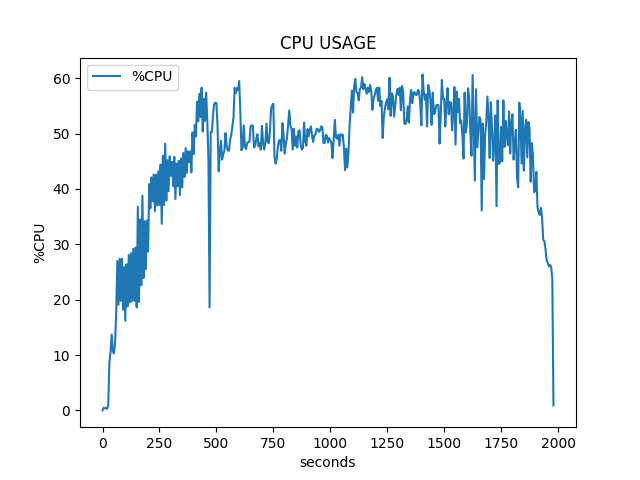
\includegraphics[width=1.0\textwidth]{Figures/StressTest.png}
    \caption{CPU usage under stress test}
    \label{fig:Figures/REALTIME_RESULT}
\end{figure}
\section{Overnight experiment}
\begin{figure}
    \centering
    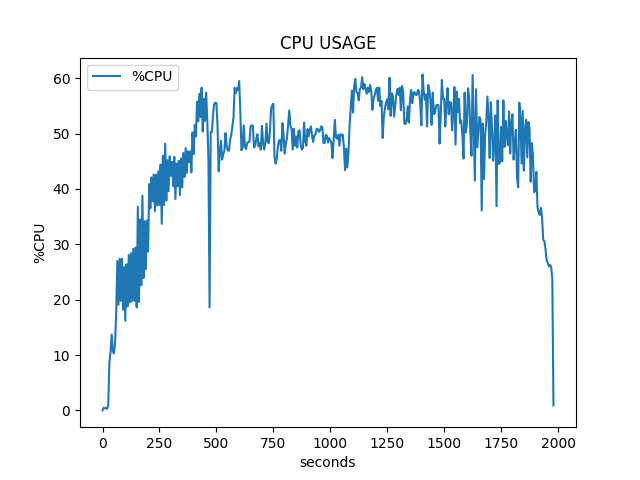
\includegraphics[width=1.0\textwidth]{Figures/StressTest.png}
    \caption{CPU usage under stress test}
    \label{fig:Figures/OVERNIGHT_RESULT}
\end{figure}
\section{EDF import}
\begin{figure}
    \centering
    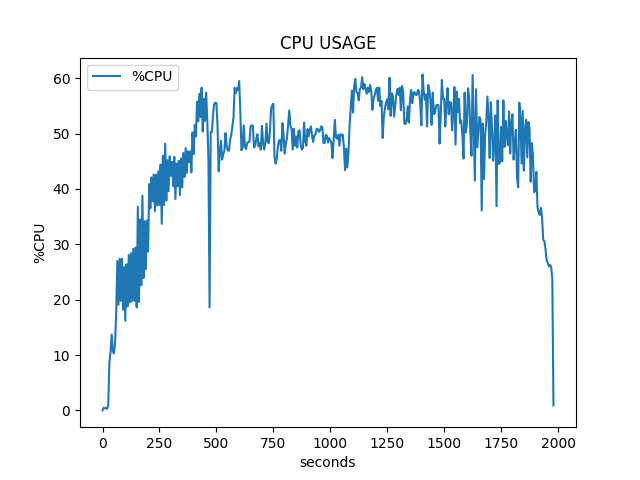
\includegraphics[width=1.0\textwidth]{Figures/StressTest.png}
    \caption{CPU usage under stress test}
    \label{fig:Figures/EDFIMP_RESULT}
\end{figure}
\section{EDF export}
\begin{figure}
    \centering
    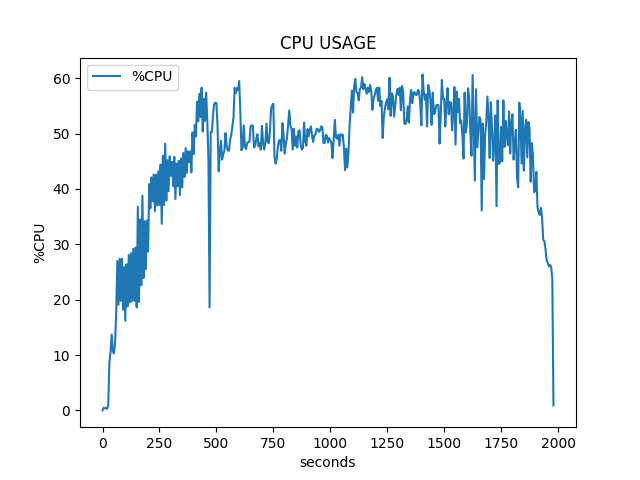
\includegraphics[width=1.0\textwidth]{Figures/StressTest.png}
    \caption{CPU usage under stress test}
    \label{fig:Figures/EDFEXP_RESULT}
\end{figure}
\section{Querying data experiment}
\begin{figure}
    \centering
    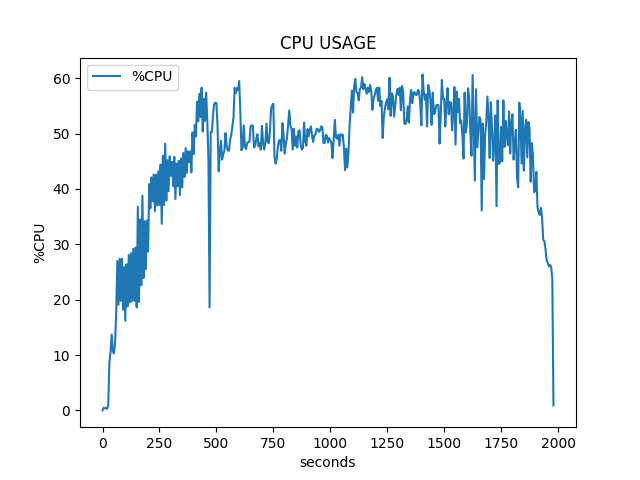
\includegraphics[width=1.0\textwidth]{Figures/StressTest.png}
    \caption{CPU usage under stress test}
    \label{fig:Figures/QUERYING_RESULT}
\end{figure}
